\documentclass[12pt]{article}
\usepackage{mathtools, amsmath, amsfonts, amssymb, siunitx,array}
\usepackage{hyperref, graphicx, wrapfig, geometry}
\usepackage[makeroom]{cancel}
\usepackage{placeins}
\usepackage{float}


\newgeometry{margin=2cm}

\title{Microprocessor Systems - Lab 4 Report}
\author{Auguste Lalande, Felix Dube, Juan Morency Trudel}
\date{\today}

\begin{document}
\maketitle
\clearpage

\tableofcontents
\clearpage

\section{Abstract}
Lab 4 encapsulates the features developed in the previous labs: pitch and roll measurement, temperature measurement, Kalman Filter, 7-segment display, user interface (keypad). In addition, an operating system is being used in order to create and manage the different threads needed for the user interface and data processing. The OS is also responsible for the inter-process communications. This system have been implemented on the STM32F4DISCOVERY board’s STM32F4407VGT6 processor using the CMSIS RTOS.

\section{Problem Statement}
The objective of this experiment is to take input from the accelerometer, the temperature sensor, and the user (through a keypad) and output some feedback on a 7-segment display in a multithreaded real time operating system (RTOS). The system has to be designed for maximum efficiency of the processor (most idle time), hence the thread should be optimized for speed. Table \ref{Table_tasks} shows the major goals of lab 4 with their associated pass criteria.

\begin{table}[!h]
\centering
\caption{Task and pass criteria for lab 4}
\label{Table_tasks}
\begin{tabular}{|p{0.5\linewidth}|p{0.5\linewidth}|}
\hline
\textbf{Task to be accomplished} & \textbf{Criteria for success} \\ \hline
Measurement of the pitch and roll angle of the development board with the accelerometer's readings. Also the accelerometer should be calibrated. & The value of the calculated angles should be within \SI{4}{\degree} of the actual physical angle measured with a protractor. \\ \hline
Use an external interrupt to signal when data is ready from the accelerometer at 25 Hz & Interrupt callback function is accessed by the software (Verified in Keil debug mode with breakpoint). \\ \hline
Read the data from the temperature sensor at 100 Hz with an ADC and convert the raw value to temperature. & Verify that the temperature is within range of the datasheet (25°-35°) and that the data is actually being polled 100 times per second (by using the Keil RTOS thread visualisation tool). \\ \hline
Set up the 7-segment display to show the temperature or the angle reading. Adjust the decimal point depending on how big the number is. & No flickering on the display. Switching between number precision with no noticeable delay. \\ \hline
Use a 3x4 keypad for user input. A button is used to change between temperature and angle visualisation on the 7-segment. Another button is used for switching between pitch and roll within the angle mode. & Any button press should be captured correctly (even fast button press) and only one key should be recorded for a long button press. No false positive should be present. \\ \hline
The system should be implemented within using the CMSIS RTOS. The program should manage multiple threads and implement safe communication between these threads. & Using Keil's RTOS thread visualisation tool, verify that all the threads are active and are being activated at their respective frequency. Also verify that most of the time (\textgreater 50 percent) is spent in idle. \\ \hline
The 7-segment display should flash when the temperature is over a certain threshold no matter which mode the display is currently in. & Verify that the display actually flashes after the threshold and stops flashing when the temperature drops down. \\ \hline
\end{tabular}
\end{table}


\section{Theory and Hypothesis}
\subsection{Accelerometer}
Accelerometers are electromechanical components used to measure the acceleration of objects. This can be useful in applications which require a precise angle such as photography, or instruments which must be held in a still position to work properly such as computer hard-drives.

Accelerometers such as the one on the discovery board are composed of springs which compress under acceleration, modifying the capacitance across them. The capacitance can then be measured and converted to a digital signal. \cite{AN3182ApplicationNote}


For this particular application, the accelerometer was set to continuously sample the acceleration and trigger a hardware interrupt when new data was available. The interrupt would indicate to the CPU that the accelerometer had finished processing data. The CPU would then call the interrupt service routine (ISR) which contained the necessary information to sample the accelerometer data.



Multiple methods can be used to calibrate any sensor. A quite common one is the least square method which is used in linear regression of an overdetermined system \cite{bjorck1996numerical}. For a 3D accelerometer, three value have to be calibrated, the x, y and z values of the acceleration. One way to apply the least square method is to measure the x, y, z acceleration at 6 known positions to then approximate the linear parameters \cite{AN3182ApplicationNote}. Once these parameters are know, this simple matrix multiplication can be applied to calibrate the raw values:
\begin{equation} \label{cal_eq:1}
 \begin{bmatrix}A_{xout} & A_{yout} & A_{zout}\end{bmatrix} = \begin{bmatrix}A_{xraw} & A_{yraw} & A_{zraw} & 1\end{bmatrix} *
\begin{bmatrix}ACC_{11} & ACC_{12} & ACC_{13} \\
ACC_{21} & ACC_{22} & ACC_{23} \\
ACC_{31} & ACC_{32} & ACC_{33} \end{bmatrix}
\end{equation}
The parameters $ ACC_{XX} $ can be calculated from measurements of 6 known positions which are 1g and -1g for x, y and z. Once the measurements are taken, the parameters can be found using the following equation:

\begin{equation} \label{cal_eq:2}
 X = (\begin{bmatrix} w^{T}*w \end{bmatrix})^{-1}*w^{T} * Y
 \end{equation}

Where the W and Y matrix are equal to:

\begin{equation} \label{cal_eq:3}
 Y = \begin{bmatrix} 0 & 0 & 1  \\
            0 & 0 & -1 \\
                      0 & 1 & 0  \\
                      0 & -1 & 0 \\
                      1 & 0 & 0  \\
                      0 & -1 & 0
                      \end{bmatrix}
\end{equation}

\begin{equation} \label{cal_eq:4}
 W = \begin{bmatrix} A_{x@z=1} & A_{y@z=1} & A_{z@z1} & 1 \\
            A_{x@z=-1} & A_{y@z=-1} & A_{z@z-1} & 1 \\
                      A_{x@y=1} & A_{y@y=1} & A_{z@y1} & 1 \\
                      A_{x@y=-1} & A_{y@y=-1} & A_{z@y-1} & 1 \\
                      A_{x@x=1} & A_{y@x=1} & A_{z@x1} & 1 \\
                      A_{x@x=-1} & A_{y@x=-1} & A_{z@x-1} & 1 \\
                      \end{bmatrix}
\end{equation}
\subsection{Keypad}
The keypad used in this lab was a simple button array with three rows and four columns. Each row and column was connected to an external pin. A button press would short one row pin with one column pin. Details on how to identify the pressed button can be found in section \ref{implementation:keypad}.


\subsection{Real-Time Operating System}
Real-Time Operating Systems (RTOS) are useful for applications which run in real time; that is to say applications which require data to be processed as it comes in. At the expense of performance, the use of an RTOS reduce development time due to hardware level abstraction and multiple function already available. An RTOS is particularly useful to split tasks into threads so that data sampling and processing can both occur continuously and with precise timing. The OS is also responsible for mutual exclusion of shared data, and inter-process communications.


\subsection{Kalman Filter}
The data gathered from the accelerometer needs to be filtered. This was accomplished using a Kalman Filter. The kalman filter equations are presented below (equations \ref{kalman_eq1} to \ref{kalman_eq4}) where q is the process noise covariance, r is the measurement noise covariance, x is the estimated value, p is the estimation error covariance, and k is the adaptive gain. More information of this filtering algorithm can be found in our previous report \cite{Lab2report}.

\begin{equation}
\label{kalman_eq1}
p=p+q
\end{equation}
\begin{equation}
k=p/(p+r)
\end{equation}
\begin{equation}
x=x+k*(measurement-x)
\end{equation}
\begin{equation}
\label{kalman_eq4}
p=(1-k)*p
\end{equation}

\subsection{Roll and Pitch Measurement}
From the accelerometer data, it is possible to calculate the roll and pitch angle of the board with constant sensitivity using equations \ref{roll_eq} and \ref{pitch_eq}, where A\textsubscript{x1}, A\textsubscript{y1}, and A\textsubscript{z1} are the acceleration for the x, y and z axis respectively:

\begin{equation}
\label{roll_eq}
Roll = arctan \Bigg( \frac{A_{y1}}{\sqrt{(A_{x1}equation)^2+(A_{z1})^2}} \Bigg)
\end{equation}

\begin{equation}
\label{pitch_eq}
Pitch=arctan \Bigg( \frac{A_{x1}}{\sqrt{(A_{y1}equation)^2+(A_{z1})^2}} \Bigg)
\end{equation}

\subsection{Hypothesis}
The complete list of requirements is synthesised in table \ref{Table_tasks}. Our team predicts that all the criteria will be achieved. Furthermore, it is believed that a precision within \SI{2}{\degree} for the roll and pitch angle can be achieved. Finally, since the program requirements remain simple, the threads should not take more than 10\% of the processor time, the remaining 90\% being idle time.



\section{Implementation}
\subsection{Accelerometer}
The accelerometer was used with a polling rate a 25Hz, a bandwidth of 50Hz, and a full scale of 2g. The accelerometer tell the microcontroller that data is ready by using a pulsed interrupt on pin 1 of GPIO port E. The interrupt is set as active high with a priority of 1. After calibrating the sensor, the acceleration data of the x, y and z axis have been filter using the Kalman Filter and then used to measure the roll and pitch angle of the board. \\

The 6 know position measurements for calibration were done using the desks in the lab space for z = ±1g. The right angle of the windows in the lab were used to position the board for the measurement of y = ±1 and x = ±1. 180 measurements (30 per position) were taken an a mean was calculated for each position. Then the parameters for the calibration matrix were extracted using equation \ref{cal_eq:2}. The calibration on the raw data was then simply implemented using \ref{cal_eq:1}

\subsection{Keypad} \label{implementation:keypad}
To detect a button press, all column pins were set to high and the value of the row pins was continuously monitored. If a button was pressed it would create a short between one column pin and one row pin which could be read by the microcontroller. The column pins were then set to high impedance and the row pins to logic high. The column pins where then checked to see which corresponded to the pressed button. Since each button corresponded to a unique pattern of column and row, the pressed button could then be identified. In order to prevent bouncing, the keypad is deactivated for a short amount of time when a key is pressed and depressed. Also when a key is pressed, the keypad is locked until it is depressed (using a variable) in order to prevent the keypad from detecting multiple key presses when the key is actually pressed only once.

\subsection{Threads}
A total of four threads were used in this lab. Details of their implementation can be seen in figure \ref{fig:threads} in the appendix.

Two of the threads were dedicated to data sampling (Thread\_Acc and Thread\_Temp). Thread\_Acc was set to sample the accelerometer data whenever data was available. Once the accelerometer had finished sampling data, it would trigger an interrupt which would make the CPU call the associated interrupt service routine, which would in turn signal the waiting thread so that it could start receiving the data. After the data received, the thread would then filter the data and calculate the pitch and roll of the board. It would then update global variables with the pitch and roll so that other threads (specifically the display thread) could use them. The temperature thread used a simpler implementation whereby it would wait a specific delay, then start the adc, wait for completion of data conversion, filter the data, convert it to temperature, and finally make it globally available; then wait for another delay before restarting the process.

One thread was dedicated to monitoring the keypad (Thread\_Keypad). This thread, similarly to the temperature thread would wait a delay then check a button had been pressed. The process for detecting button presses is detailed in section \ref{implementation:keypad}. If a push was detected, the thread would switch some global flags indicating to the display thread what actions to take. If not it would wait another delay before checking again.

The last thread (Thread\_Segment) was in charge of updating the 7-segment displays. This thread also functioned using osDelays, although the delay had to be much shorter then in the other threads so that no flickering would occur. The purpose of this thread was twofold, it first checked the flags set by the keypad thread to decided which of the temperature, the pitch ,or the roll needed to be displayed. It then checked the alarm flag set by the temperature thread (indicating whether or not the CPU was overheating), to determine if the display should start flashing. Details on operating the 7-segment displays can be found in our previous lab report \cite{Lab2report}.

\section{Testing and Observations}
Multiple criteria were met directly by having a fully functional system and looking at the output on the 7-segment display and in the debug (printf) viewer. Also, by using checkpoints to verify if the code was branching to the right place at the right moment (e.g. interrupt the accelerometer data conversion), correct code behaviour was verified. Additional tests were conducted for the 7-segment, the Keypad, the accelerometer, and the thread timing.

\subsection{7-Segment Display and alarm}
All the testing of the 7-segment and the alarm was done by simply looking at the display and verifying that all 3 members could not detect any flickering or other timing problems. The display was then left on for a minute to see the consistency of the implementation. The alarm was triggered and stopped 5 times without fail.
\subsection{Keypad}
The Keypad was tested to make sure all button press output were interpreted as the right character, that the fastest user input was detected and that slow user input was detected only once. The longest user input tested was 10 seconds long recorded with a chronometer and the shortest was 0.15 seconds. After more than 10 samples for every key, no problems or error were detected on the final system.

\subsection{Accelerometer}
The precision of the accelerometer was assessed by measuring the board's angle with a protractor and comparing with the value displayed on the 7-segments. 5 Measurements were done for pitch and roll at 0, 45 and 90 degrees and their respective mean values are reported in table \ref{Table_acc_roll} and table \ref{Table_acc_pitch}. Note that the measured angles had a limited precision to about \SI{1}{\degree} due to human error.

\begin{table}[!h]
\centering
\caption{Mean roll angle measurements at \SI{0}{\degree}, \SI{45}{\degree} and \SI{90}{\degree}}
\label{Table_acc_roll}
\begin{tabular}{lllll}
\hline
\textbf{Degree} & \textbf{0} & \textbf{45} & \textbf{90} & \textbf{Mean Error for Roll}
\\ \hline
\textbf{Before Calibration} 2.9 & 46.8 & 92.7
\\ \hline
\textbf{Mean Error Before Calibration} & 2.9 & 1.8 & 2.7 & \multicolumn{1}{c}{\textbf{2.47}}
\\ \hline
\textbf{After Calibration} & 0.5 & 45.6 & 89.0
\\ \hline
\textbf{Mean Error After Calibration} & 0.5 & 0.6 & 1 & \multicolumn{1}{c}{\textbf{0.7}}
\\ \hline
\end{tabular}
\end{table}

\begin{table}[!h]
\centering
\caption{Mean pitch angle measurements at \SI{0}{\degree}, \SI{45}{\degree} and \SI{90}{\degree}}
\label{Table_acc_pitch}
\begin{tabular}{lllll}
\hline
\textbf{Degree} & \textbf{0} & \textbf{45} & \textbf{90} & \textbf{Mean Error for Pitch}
\\ \hline
\textbf{Before Calibration} & 1.93 & 45.6 & 88.2
\\ \hline
\textbf{Mean Error Before Calibration} & 1.93 & 0.6 & 1.8 & \multicolumn{1}{c}{\textbf{1.44}}
\\ \hline
\textbf{After Calibration} & 0.9 & 44.8 & 90.5
\\ \hline
\textbf{Mean Error After Calibration} & 0.9 & 0.2 & 0.5 & \multicolumn{1}{c}{\textbf{0.53}}
\\ \hline
\end{tabular}
\end{table}

\newpage

\subsection{Thread timing}
Thread timing was verified using the Keil event viewer thread visualisation tool (figure \ref{fig:threadstiming}). The execution time for each thread was measured using this tool and is reported in table \ref{Table_threads}. As can be seen from the table, 97.74\% of the time is spent in idle state which is far more than our hypothesis.

\begin{figure}[!h]
 \centering
 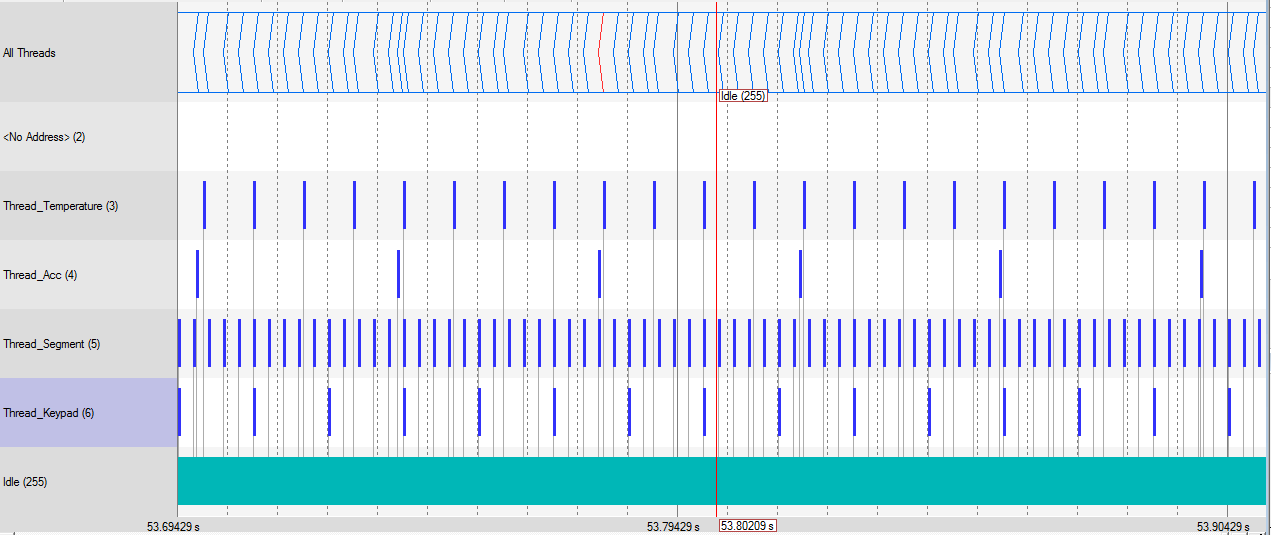
\includegraphics[scale=0.50]{images/threads1.png}
 \caption{Thread Timing Diagram}
 \label{fig:threadstiming}
\end{figure}


\begin{table}[!h]
\centering
\caption{Execution time and frequency for each thread}
\label{Table_threads}
\begin{tabular}{|l|c|c|c|}
\hline
\textbf{Thread} & \multicolumn{1}{l|}{\textbf{Execution time ($\mu s$)}} & \multicolumn{1}{l|}{\textbf{Frequency ($Hz$)}} & \multicolumn{1}{l|}{\textbf{Total time per second ($ms$)}} \\ \hline
Temperature & 50 & 100 & 5.00 \\ \hline
Acceleration & 130 & 25 & 3.25 \\ \hline
7-Segment & 40 & 341 & 13.64 \\ \hline
Keypad & \textless10 & 67 & 0.67 \\ \hline
Idle & \textgreater977440 & 1 & 977.44 \\ \hline
\end{tabular}
\end{table}

\newpage

\section{Conclusion}
The use of an RTOS allowed the system to concurrently sample the CPU temperature, sample the accelerometer, display some value on the 7-segment display, and poll the keypad for user input. As the results suggest all the features could be done at specific frequencies without one thread affecting another's functionality. The 97,7\% mean idle time exceeded our expectations.    This shows that the use of an RTOS in this scenario is justified because simplicity was more important than performance.

\newpage
\section{Bibliography}
\bibliographystyle{unsrt}
\bibliography{LabReport4}

\newpage
\section{Appendix}
\begin{figure}[!htb]
 \centering
 \includegraphics[scale=0.40]{images/threads.png}
 \caption{Threads Diagram Representation}
 \label{fig:threads}
\end{figure}

\end{document}
